\documentclass[runningheads]{llncs}
\usepackage{graphicx}
\usepackage{comment}
\usepackage[colorinlistoftodos]{todonotes}
\begin{document}
\title{Blockchain in the Industrial Sector}
\institute{
RWTH Aachen University, Germany \\
\email{mohammad.ghanem@rwth-aachen.de}}
\author{Mohammad Ghanem}
\maketitle

\let\labelitemi\labelitemii

\section{Introduction}

\subsection{Motivation}
Until today, the industry has seen three major revolutions, and the fourth is on its way \cite{Rojko2017}. The fourth industrial revolution (Industry 4.0) represents the next step in the evolution of traditional factories towards smart automated factories. These factories are designed in such a way to reduce production costs, increase productivity, improve quality, and achieve efficient use of resources. To achieve all that a wide range of technologies have to be used in manufacturing processes like Robotics, Autonomous Systems, Internet of Things, Cloud Computing, Intelligent Data Analytics, Artificial Intelligence, and many more \cite{Fernandez-carames2018}.

\bigbreak

\noindent However, all these technologies are relying on centralized networks and need to trust middlemen or third-party operators \cite{Angrish2018a,Sikorski2017,Li2018,Afanasev2018,Garrocho2019}. As a result, the industry is facing many challenges related to the data. Challenges like transparency, security, privacy, and trustworthiness. These challenges prevent Industry 4.0 to reach its full potential. A decentralized and trusted platform is needed to facilitate the relationships among parties across the value chain. Such a platform can be built with the help of blockchain technologies.

\bigbreak

\noindent The main  advantage of the blockchain is decentralization. It is a distributed shared ledger instead of the traditional centralized systems \cite{Zheng2017}. It enables a group of entities to reach an agreement on a certain activity and register it without the need for a middleman or third party. The agreed-upon activity can be anything like payment transactions, purchase activity, or any non-financial transaction \cite{Mohamed}. The great revolution blockchain brought by creating an immutable, secure and transparent system to log and execute any type of transaction. Blockchain can also preserve the order of events and ensure the correctness of logged transactions over time. No one can individually delete or modify any of the recorded transactions. Also, the invention of smart contracts made the blockchain a promising platform for developing distributed and trustworthy applications \cite{Mohamed}. As a result, many industries and businesses are considering its utilization and more research is being done to effectively apply blockchain in their domains.

\bigbreak

\noindent Given its key features such as immutability, traceability, and reliability of the information, it represents a perfect candidate to be integrated into the industrial plants. It will increase its efficiency, security, and provenance concerning the related data of goods, assets, and operations \cite{Internet2019}. In addition, these features enable the creation of new business models that were impossible to form a few years ago. With the introduction of blockchain, businesses and individuals can record and secure their conducted agreements among themselves without middle parties.


\subsection{Problem Statement}
In the manufacturing industry, many technologies are evolving. They all have the same goal in increasing the efficiency, capability, and adaptability of the manufacturing systems. However, all technologies rely on a centralized network provided by a third party. This limits the ability of these technologies to achieve their goal and limit the scalability of the manufacturing systems. Also, it imposes vulnerabilities as cyber-attacks and security problems.


\subsection{Research Purpose and Questions}
The aim of this thesis is to shed light on the blockchain’s capability to improve the manufacturing industry. It will investigate the feasibility of implementing blockchain solutions within the boundaries of smart factories. To understand how blockchain can work with other technologies to overcome the challenges mentioned earlier. The main question for this research is:

\paragraph{Can blockchain and smart contracts technologies be used as a basis for other manufacturing technologies?} To answer this main research question, this research will address several sub-questions:
\begin{itemize}
  \item Why should blockchain be implemented inside factories? (The benefits?)
  \item Which are the manufacturing subareas that can benefits from blockchain?
  \item What are the approaches for implementing such blockchain-based solution? 
  \item What are the challenges for implementing such blockchain-based solution? 
\end{itemize}

\subsection{Outline}
The remainder of the document is structured as follows. Section 2 presents an overview of the research that has been made in the fields of blockchain for the manufacturing industry. In the next section, we provide an overview of the system requirements and functionalities. Then section 4, discusses some technical details about the proposed system implementation. Later in section 5, a short section about the system evaluation. Finally, the last section summarizes the document. 

\newpage

\section{Related Work}
The topic of this thesis involves two domains, the manufacturing industry, and the blockchain technology. To identify the relevant existing work, we had to look for research that has been done in the manufacturing area in general and the work involves applying blockchain technology. Our search was on the popular academic search engines such as Google Scholar, arXiv, and Research Gate. We searched for the following terms: ("Blockchain" OR "Distributed Ledger" OR "Smart Contract") AND ("Manufacturing" OR "Production" OR "M2M" OR "Factories" OR "Plants").  The result of our search included research papers published in journals and conferences. During the identification and selection process, we found several technologies are being used in the manufacturing industry and can be integrated with blockchain. Many researchers have already introduced blockchain-based applications to each one of these technologies. The main technologies are cloud manufacturing and machine-to-machine communication.  
\bigbreak

\noindent
In the following subsections, we will describe what we found the most relevant to the discussed problem. For each one of the studies, we are describing the goal behind the work, the implementation approach, and the prototype if available. 

\subsection{FabRec: A Prototype for Peer-to-Peer Network of Manufacturing Nodes \cite{Angrish2018a}}

In this work, the goal is to build a trustless distributed network. Where different industrial organizations can collaborate and share information about manufacturing processes. The network was built using blockchain and smart contracts technologies. They stored information about machines, manufacturers and their capabilities. Through this network, all the information is shared transparently among participants. This will give a third party the ability to verify a certain capability of one manufacturer. The verification is done through a trial of past historic. This will help to make paperless contracts among participants using smart contracts. A participant of this network can be a human, manufacturing machine, a computing node, or an agent representing any organization. The information about the machine's events stored as transactions. Three types of information exist machine asset information, machine utilization, and machine capabilities. Other types of information like manufacturing related data is stored inside the state variables of the smart contracts.  They designed three 3 smart contract representations to represent the relationships between various participants of the network.
\bigbreak

\noindent
The prototype of this work was a small network built using Ethereum. To how machines on a decentralized network can autonomously interact without human involvement. The network consistent of 4 separate computers representing various fabrication service providers and two mining nodes. To simulate the machines, they used Arduino and a CNC machine controlled through MachineKit\footnote{https://www.machinekit.io/} interface. The setup was intended to demonstrate how a smart contract can check for certain events received by the CNC machine. Then the contract triggers a command sent to the Arduino board. The work also evaluates the performance of the prototype for two types of consensus algorithms: proof of work (POW) and proof of authority (POA). The evaluation used two metrics. The first one is the time it takes for a transaction to be included in a block on the blockchain. The second one is the time the block takes to reach a certain number of confirmations in the chain.
\bigbreak

\noindent
We think this work focused more on the horizontal integration of technology among many manufacturers.  The network does not contain data about the manufacturing process. Such data is being accessed through oracles from other existing Enterprise Resource Planning (ERP) systems and Manufacturing Execution Systems (MES). The work assumed that these existing IT systems are trustworthy. Regarding the prototype, it did not take into consideration a full automated manufacturing scenario. However, they showed through the prototype the autonomous decision making and interaction of two physical devices on the blockchain network.  

\subsection{Toward a blockchain cloud manufacturing system as a peer to peer distributed network platform\cite{Li2018}}


The authors of this work integrated cloud manufacturing technology blockchain. The goal was to build a distributed peer to peer network architecture. To improve the security and scalability of cloud platforms used by manufacturing service providers. They proposed an architecture that provides a secure and distributed service sharing and trustable connection between end-users and service providers. Also, it provides the ability for self-trust, data integrity audit, data resilience, and secure data sharing. The architecture is made up of five layers namely; resource layer, perception layer, manufacturing layer, infrastructure layer, and application layer. They used smart contracts to write the rules of the agreement between the end-users and the service providers. These rules can contain the due date, quality measurement, and payment information.
\bigbreak

\noindent
To demonstrate the implementation of proposed architecture. The authors showed a case study which includes five manufacturing service providers and 15 end users. Each service providers can provide three types of service namely; machining as a service, the technical issue as a service and welding as a service. The end users can send one request to the system at a time. The scenario begins when a customer wants to produce an industrial piece that can be manufactured with a CNC milling machine. He published information about the piece using the blockchain smart contract. Then, service providers send their offers to the customer (product cost and due date). When the customer accepted an offer from the service provider, it is executed as an atomic exchange. To simulate the physical machines they used CNC simulator \footnote{\url{https://cncsimulator.info/}}. They used MultiChain as blockchain platform. In addition, a security and performance evaluation was carried to verify the proposed architecture. They discussed three security requirements, namely: confidentiality, integrity, and availability. The performance evaluation is done based on wallet creation time and data encapsulation operation on the blockchain. \bigbreak

\noindent
We think the focus of this work was on building a trusted peer to peer network to enable manufacturing as a service. The aim was to enhance communication between manufacturing parties. To overcome the issues resulted from the centralization. The main benefit of using the blockchain in this work to enable secure data exchange. However, this work didn't take into consideration how architecture can be used to automate the production process itself. \bigbreak

\noindent
A similar approach was presented in \cite{Barenji2019}. The goal also was to improve communication between manufacturing services users and manufacturing services providers. The proposed platform is explained in detail based on its architecture, consensus mechanism, and communication protocol. The use case of this work was in 3D printing manufacturing. They tested based on network performance and three practical scenarios. The results show that blockchain technologies can help to solve some existing problems found in the literature of cloud manufacturing. 


\subsection{BPIIoT: A Light-Weighted Blockchain-Based
Platform for Industrial IoT \cite{Bai2019}}
The work addresses the security, trust, and island connection problems in the Industrial IoT (IIoT) ecosystem. The proposed architecture consists of two parts on-chain network and off-chain network to reduce network load and latency. The on-chain part provides data communication and transmission services. Whereas, the off-chain provides data storage and complex processing which can't be done in the on-chain part. In this platform, any machine/equipment can add operation data to the blockchain, send transactions to the related smart contracts, and receive transactions from other nodes in the blockchain. Two applications discussed in detail to demonstrate the proposed architecture.\bigbreak 

\noindent 
One of the applications is smart predictive maintenance. Where the platform can be used to manage the equipment information and the maintenance process. The shown use case was about packaging platform based on the proposed BPIIoT architecture. It has two sensors connected with two robots to collect state data, such as temperature and vibration. This state information is being recorded in the on-chain network. The smart contract which serve as agreement between the equipment owner and the maintenance service provider, is monitoring the state information. When the temperature or vibration frequency exceeds a given threshold for a certain number of times, a command is triggered by the smart contract. In this way, the equipment can request for maintenance services, replenishment or replacement of spare parts issued by the service provider/supplier. The did not present the technical details about the implementation of this application. Overall this work did not focus on the internal manufacturing processes. 

\subsection{Blockchain technology in the chemical industry: Machine-to-machine electricity market \cite{Sikorski2017}}

One of the most highly cited papers with more than 250 citations. It is one of the first research works which used the M2M concept with blockchain. In this paper, the authors explored the applications of blockchain in relation to Industry 4.0. They build a proof of concept where a blockchain is used to facilitate the interaction between machines. The goal was to enable M2M electricity market. Where industrial plants are autonomously trading electricity with each other over a blockchain. The agreement between the producer and the consumer is done using smart contracts. Information about the energy consumption (in kWh) published by the machines stored as transactions in the blockchain. Each transaction as a fee (in USD) according to the agreement specified by the smart contract. \bigbreak

\noindent In their prototype, the scenario presented includes two electricity producers and one electricity consumer trading with each other over a blockchain. The physical machines were replaced with simulations of industrial processes in Aspen Plus (AP) \footnote{\url{https://www.aspentech.com/en/products/engineering/aspen-plus}}. They used MultiChain \footnote{\url{https://www.multichain.com/}} to build the private blockchain. The authors did not evaluate their prototype. The focus of this work was on energy trading using M2M. The work doesn't provide any sort of framework or architecture that can be used on a large scale in manufacturing. This work was only to demonstrate that the blockchain can be used to facilitate the interaction between machines. \bigbreak 

\noindent Another work in the M2M domain is presented in \cite{Afanasev2018}.  The goal is to use BC and smart contracts to build a decentralized network for secure M2M communication within cyber-physical production systems (CPPS). The authors discussed three blockchain network architectures. They showed their main features and limitations. Based on their discussion, Ethereum blockchain with proof of stake is the most suitable architecture for a CPPS backbone network. In this paper, the authors did not present an actual implementation. The use case was about printed circuit boards (PCBs) production. They discussed it in theory without any technical details.  Showing how PCBs can benefit from the proposed architecture.
 
\subsection{Industry 4.0: Smart Contract-based Industrial Internet of Things Process Management \cite{Garrocho2019}}

In this study, the authors focused on the industrial machine to machine communication and how it can be improved by blockchain technologies. They introduced smart contract-based middleware for M2M communications to make it secure and decentralised. Through this middleware, IoT devices can communicate without the need or a trusted intermediary. Industrial Smart Contract Monitor (ISCOM) is the name of the middleware. It controls and executes contracts to order tasks from field devices. ISCOM monitors the field device states and executes actions based on a change in their state. It may also request a field device to perform service under a smart contract. All information about the actions and processes are recorded in the blockchain through smart contracts. 

\bigbreak

\noindent
 The authors present a proof of concept to simulate smart contracts in the industrial context. They used two Raspberry Pi 3 boards representing field devices. MQTT server for the communication between devices. For the blockchain network and smart contract implementation, the Ropsten Ethereum test network was used. The proof of concept worked in such a way that after the device changes its state, it publishes this change to the MQTT server. The middleware subscribes to the device publications and reviews the state according to the deployed smart contracts. Once the conditions of a smart contract satisfied, The middleware publishes messages to request a service from another field device. The other device picks this message published by the middleware and executes the operation accordingly. Two experiments were performed to evaluate the impact of latency and blocking time. The blocking time is the response time of the sensor device requests a change in the state of the smart contract.  The latency time is the delay time leading to communication between field devices and ISCOM. The experiments showed a high and variable blocking time for smart contracts. Which makes them unsuitable for M2M real-time communications. 

\bigbreak

\noindent
Unlike the other works, the focus here was on vertical communication within one factory. This work emphasises on the real-time requirement for M2M communications in industrial processes. The result showed that the smart contracts technology is still not mature enough to provide such essential requirement. Similar to the other works, the proof of concept was small and limited to only two devices. 



\subsection{Summery}
It is evident from the works we discussed in this section that researchers have already presented some applications of blockchain in the manufacturing industry. The approaches as we saw vary wildly and each work looks at the problem from a different angle. Some of the works focused on the horizontal integration between manufacturing parties to enable the concept of manufacturing as a service. Either between manufacturers themselves or between manufacturers and customers. These works neglected the actual manufacturing process and focused more on the concept of trading. On the other hand, some works discussed the manufacturing process by enabling machine-to-machine communication over the blockchain. However, the use cases of these works were oversimplified and in most cases were limited in size (two machines). This does not reflect the actual communications between machines on a production line. The majority of the discussed works did not store information about the manufactured products. To overcome these points, we propose our solution in the next section.


\section{Proposed Solution}
To answer the research questions, we will try to build a blockchain-based system in the area of manufacturing. The system collects, stores, and manages the key information generated by the factory infrastructure. The focus is on both the machines and the products being manufactured. Regarding the products, the system provides the ability to track and trace each product throughout a production pipeline. Regarding the machines, it tracks the status of the machines at any point in time. The system enables also the autonomous machine-to-machine communications. Where one machine can ask another machine to perform a certain task without any human involvement. The system envisioned will be designed and implemented using blockchain technologies such as smart contracts. It will be decentralized and distributed. The system will be serving the entities participating in the manufacturing industry such as suppliers, manufacturers, and customers. 

\bigbreak 

\noindent In the system, each machine and product has a digital profile. The profile of the product contains all related information about how the product has been manufactured. The profile will contain the full log of all the industrial tasks performed to this product. This includes information about the machines performed the tasks and information about the surrounding environment. Each product will have an information tag attached to it to serve as a digital identity. This can be a barcode or RFID. The tag will serve as an identifier linking the physical product with its virtual twin on the network. The profile of the machine will contain related information about the industrial tasks performed by this machine and information about the communication with other machines. All the data in the network is stored on a blockchain and is available to anyone running the system software with correct authentication.

\bigbreak

\noindent The system consists of several types of actors:
\begin{itemize}
  \item Registrars – provides unique identities to other actors on the network.
  \item Manufactures - own the machines of the factory.
  \item Suppliers - provide the raw materials for the factory.
  \item Customers - purchase the manufactured products.
\end{itemize}

\noindent Actors will also have their own digital profile on the network, which is created upon registration. Upon registration,  public and private cryptographic key pair are generated for each actor. The public key identifies the actor within the network and the private key authenticates the actor when interacting with the system.

\section{Implementation}
The figure \ref{fig:system_overview} shows a high-level overview of the system compounds. The system consists of two main parts. The blockchain part, which is a private permissioned blockchain with a set of deployed smart contracts. The factory part is the infrastructure of the factory with all the machines and sensors. These two parts are communicating using Message Queuing Telemetry Transport (MQTT) protocol through the MQTT broker. MQTT is an open message protocol that enables the transmission of data in the form of messages between devices. The following sub-sections will explain each compound in detail.

\begin{figure}
\centering
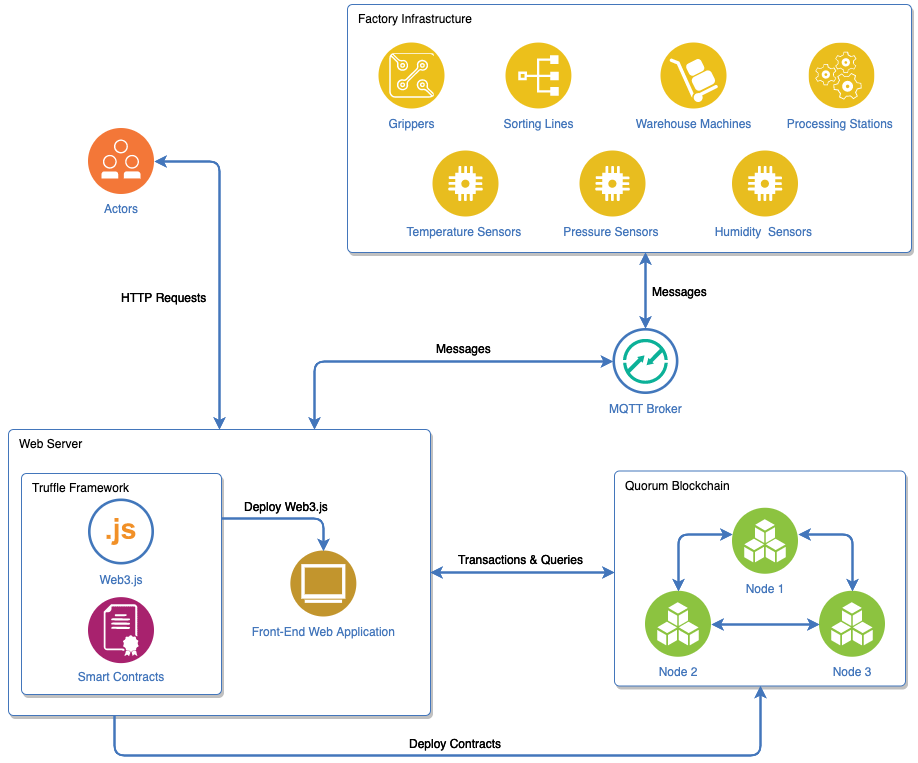
\includegraphics[width=1\textwidth]{figures/system_overview_2.png}
\caption{High Level System Overview}
\label{fig:system_overview}
\end{figure}

\subsection{Factory Infrastructure}
This includes different types of manufacturing resources like machines and sensors. We assume that all resources are able to communicate using MQTT protocol. Each resource can send and receive messages with a certain topic. The messages sent by resources will be forwarded through the MQTT broker to a web application. Then it will send the corresponding transactions to the blockchain.

\bigbreak

\noindent To simulate such infrastructure in our implementation, we are using Fischertechnik \footnote{https://www.fischertechnik.de/} factory model. It is a simulation of a factory used for learning and understanding industry 4.0 applications. It depicts the ordering process, the production process, and the delivery process in digitised and networked steps \cite{Industry}. It consists of several modules like storage and retrieval stations, vacuum suction grippers, high-bay warehouse, multi-processing station with kiln, sorting line with color detection, environmental sensor, and pivoting camera. The modules are managed by six controllers. All of them networked within the factory and communicate with each other via MQTT.

\subsection{MQTT Broker}
An MQTT broker receives the messages from the factory and forwards it to the web application. In the actual implementation, we will use the broker provided by the Node-RED server \footnote{https://nodered.org/} but any other broker can be used.

\subsection{Front-End Web Application}
This is just a front end application used to communicate with the blockchain. It can be hosted locally or in the cloud. The application uses standard front end technologies to build the user interface. To interact with the blockchain, it will use the Web3.js library \footnote{https://github.com/ethereum/web3.js/}. It is an Ethereum Javascript API implements the JSON-RPC protocol to connect and interact with any Ethereum blockchain network. This application servers two proposes. The first one is to act as a broker between the blockchain and the MQTT broker as the former can not connect directly to the blockchain. The second is to allow the actors to interact with the system. 


\subsection{Truffle Framework}
This is not an actual active compound of the system. Truffle \footnote{https://github.com/trufflesuite/truffle} is a development framework. Truffle is a development environment, testing framework, and asset pipeline for Ethereum. It allows easy compiling, deploying, and testing of smart contracts written in Solidity. Truffle is built on the top of web3.js and provides many other functionalities. This framework will be used to deploy smart contracts into the blockchain. Also, it will be used to deploy the web3.js code of the web application. 


\subsection{Quorum Blockchain}
For the implementation of this thesis we are using the Quorum \footnote{https://www.goquorum.com/} blockchain. It is a permissioned implementation of Ethereum. It has several advantages over public Ethereum like privacy, high performance, and support multiple consensus algorithms. As Ethereum, Quorum uses standard Solidity for writing smart contracts.

\section{Evaluation}
The qualitative evaluation of the proposed solution will be achieved by showing that the system is actually working. This includes details about implementation and how they comply with the proposed specifications and the requirements. Then the quantitative evaluation will be presented by analyzing the performance of the system and its scalability. Another important quantitative measure in the blockchain-based system is the cost measured by gas consumption. The pricing of gas has been removed from Quorum blockchain because it is a permissioned blockchain. However, the concept of the gas itself remains and could be measured. 

\section{Conclusion}
In this document, we presented a proposal for a decentralized tracking system for the manufacturing industry. The system is utilizing blockchain technologies such as smart contracts to overcome the challenges caused by the centralization of traditional manufacturing systems. To be continued... 

\newpage
\bibliographystyle{splncs04}
\bibliography{ref.bib}

\end{document}